\chapter{Literature Research}
\label{ch:literature}

In the following HCI research in the field of autonomous vehicles and state of the art in interfaces for autonomous vehicles are investigated. An introduction to autonomous vehicles can be found in a book by \citet{Lipson:2017:DIC:3175814} and a comprehensive overview of the current state of art in 'Human-Machine Interaction for Vehicles' can be found in a chapter by \citet{Kun2018} too. Here the most relevant literature out of more than 220 scientific articles is presented. 

\section{Autonomous Vehicle History}\label{sec:history}
Current major developments of vehicle technology are in-vehicle crash avoidance systems that provide warnings or limited automated control of safety functions; Vehicle to Vehicle (V2V) communications that support various crash avoidance applications; and self-driving vehicles. 

Most of the current autonomous concept cars show ideas that were already envisioned by century-old science fiction literature or movies. For example the Movie iRobot shows an autonomous vehicle with a steering wheel that retracts only if needed \footnote{\url{https://blog.audi.de/concept-cars-der-audi-rsq/} \& \url{https://www.youtube.com/watch?v=tY49M1F2CsA}}, KITT from Knight rider shows both a voice interface and LED communication with pedestrians\footnote{\url{https://www.2025ad.com/latest/driverless-cars-in-hollywood/}}, Total Recall has autonomous vehicles with a cab driver avatar called Johnny Cab\footnote{\url{https://talkingpointz.com/johnny-cab/} \& \url{https://www.youtube.com/watch?v=eWgrvNHjKkY}}. In old book illustrations for science fiction novels autonomous vehicles without steering wheel and seats facing each other can be seen \citep{Radtke1974DieMorgen}. Furthermore, concepts such as platooning, dedicated freight vehicles and entertainment within autonomous vehicles were already explored more than 40 years ago. 

\subsection{Levels of autonomy}\label{ssec:levels}
A few alternative classifications of vehicle automation exist. Among the most popular are the one by NHTSA and SAE. The \citet{SAEinternational2016} distinguishes six different levels whereas the older definition from the American \cite{NHTSA2013}  distinguishes between five different levels. In \emph{\fullref{fig:SAE}} the different autonomy levels are depicted. 

Most deployed vehicles operate without any automation (Level 0); even if they have functionality such as cruise control, automatic gear shifting or warning systems such as blind spot or collision warning this is not considered as automation as long as the vehicle does not intervene by itself. 
New fully equipped vehicles will often have some driver assistance functions such as adaptive cruise control (ACC) or lane keeping assist (level 1). If both steering (lane centering) and acceleration/deceleration (ACC) carried out by the vehicle but the driver has to monitor and be able to respond at all times this can be classified as partial automation (level 2). If the system is capable of driving autonomously under some conditions (e.g., on well-marked highways) and the driver does not need to monitor at all times this is classified as conditional automation (level 3). The additional distinction which SAE introduces is between high automation (level 4) and full automation (level 5). Vehicles with high levels of autonomy do not require human intervention, but they cannot drive under all roadway conditions. Vehicles of level 4 and higher thus might not need a steering wheel at all. These vehicles could be used for public transport with dynamic pick up locations. For comparison: Waymo, an Alphabet (Google) subsidiary, claims that their autonomous cabs already operate on SAE level 4 \citep{Waymo2018DriverlessApplication}. 

This thesis concentrates on autonomous cabs with high levels of automation. Neither is the passenger the owner of the vehicle, nor has he to intervene at any point during the ride. These types of vehicles seem to be way ahead in the future but in fact vehicles without access to driving controls for the passengers can already be deployed with vehicles up from conditional automation (level 3). In this case, human operators could guide the vehicle through sections of uncertainty; these operators do not even have to be physically inside the vehicle but could teleoperate it \citet{Hollander2016TheSystems}.  

\begin{figure}
    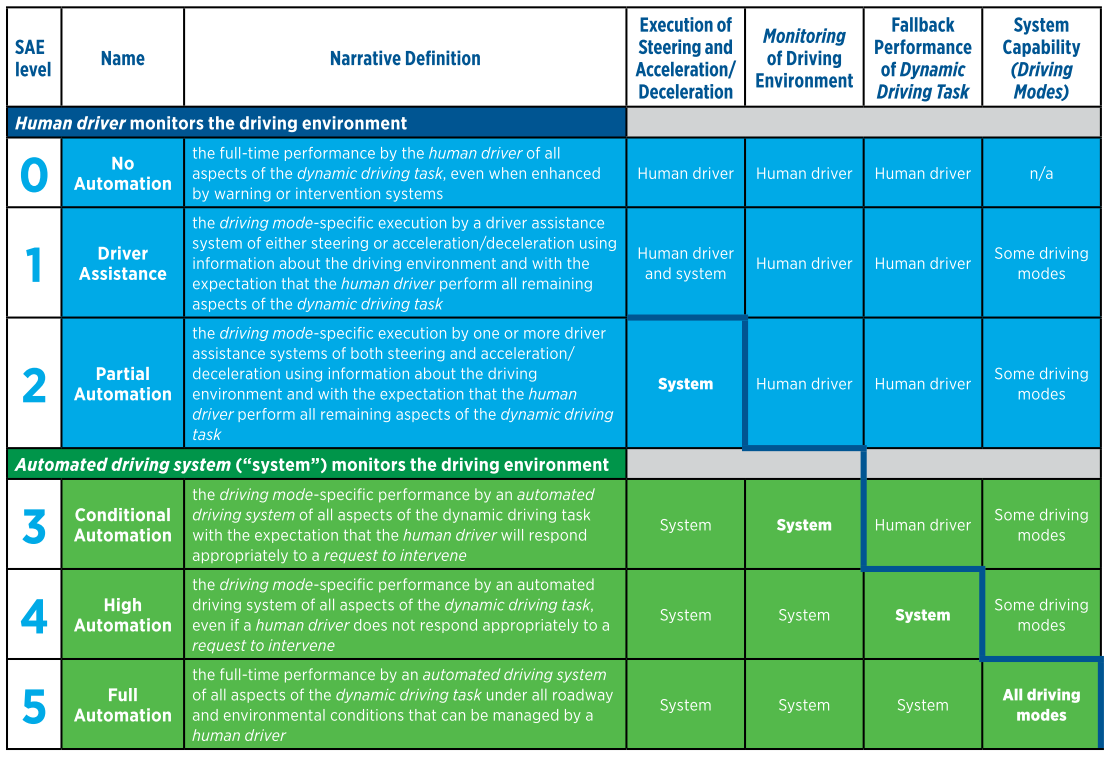
\includegraphics[width=1\textwidth]{fig/SAE}\hfill\
    \caption[SAE international automated driving levels]{SAE international automated driving levels. Figure from \cite{SAEinternational2016}}
    \label{fig:SAE}
\end{figure}

\section{Semi-Autonomous Vehicle Interfaces}
\subsection{Driver assistance technology}
A lot of assistance technologies, which are marketed differently by each automotive manufacturer, exist. A good visual overview is provided online\footnote{\url{http://mycardoeswhat.com/}}. Most assistance technologies try to increase safety. Only a few, such as automatic parallel parking, tackle convenience. As of now most of these systems work independently, in the future, these systems must work together to achieve full and semi-autonomous driving. For example, a vehicle could use obstacle detection in combination with pedestrian detection, lane keep assist, adaptive cruise control, and curve speed warning to drive autonomously; then use the drowsiness alert to detect if the driver still pays attention to the road during the self-driving time and finally use automatic emergency braking if the driver fails to intervene by himself. 

\subsection{Help the driver interfaces}
Before fully autonomous vehicles get deployed, the driver receives more assistance from the vehicles by assistance technology. There is technology that intervenes automatically and technology that just warns. For example, the vehicle could apply the brakes on its own if it detects a collision or it could play a warning sound. To help the driver there are both industry solutions, such as blind spot warning systems, and research papers from the HCI community:  \citet{Loecken2015} explored ambient light to warn of vehicles in the blind spot, \citet{Langlois2013} tested a prototype of a head-up display to communicate multiple messages from the driver assistance systems (Blind spot warning (BSW), lane departure warning (LDW), Forward Collision Warning (FCW)) by a peripheral display, \citet{Kim} and \citet{Langlois2016} tested augmented reality (in simulators) to make people aware of pedestrians and vehicles in dangerous scenarios. 
\citet{Larnaout2013} and \citet{Abdi} worked on the mapping of augmented overlays into the real scene. 

\subsection{Hand over of control}
For vehicles that are not yet fully autonomous but can drive autonomously in a few scenarios (SAE 2-3), the vehicle has to indicate when the driver needs to take back control. Humans stop actively driving the vehicle and start to monitor the autonomous system, unfortunately, research suggests that humans are not good at monitoring \citep{Naujoks2014TheConditions.}. It is difficult for humans to pay attention to tedious tasks for a long time. Moreover, driver assistance systems can be experienced as a loss of control and competency as well as a feeling of being at the mercy of technology \citep{Eckoldt2012AnSystems}. Tesla vehicles, which already employ a few self-driving functionalities (Adaptive Cruise Control (ACC), Lane Keeping Systems (LKS), Auto Lane Change (ALS)), make a rapid beep noise when the driver needs to take over control. However, two Tesla drivers died already because of inattentiveness while having autopilot turned on\footnote{\url{https://www.bloomberg.com/news/articles/2018-03-31/tesla-says-driver-s-hands-weren-t-on-wheel-at-time-of-accident}} and another one was caught sleeping\footnote{\url{https://www.theverge.com/2018/4/29/17298750/tesla-autopilot-british-driver-charged-driving-sleeping}}. Normally, the driver needs to touch the wheel to keep Autopilot active, however there are dangerous modifications sold that keep Autopilot steadily turned on\footnote{\url{https://www.autopilotbuddy.com/}}. These issues are still a field of active research. \citet{Politis} found that multimodal warnings are superior to unimodal warnings and reduce take over time, \citet{Merat2014TransitionVehicle} found that take over times are shorter when the vehicle requests them more regularly, and \citet{Koo2015} found preference for messages that describe why an event happened over how it was addressed (e.g. “Obstacle ahead” vs. “Emergency braking”).  \citet{Walch2017} give an extensive overview over current hand-over and collaboration strategies, they highlight in particular the importance of multimodality, adaptation of the system to the driver and conclude that the driver and vehicle should work as a team. \citet{Meschtscherjakova} dive into the issue that more automation means inferior driving skills. \citet{Rodel} suggest that trust in semi-autonomous vehicles (SAE-3) will be the lowest among the different automation levels because hand-over scenarios are not likely to be satisfactorily solved. 



\subsection{Ambient displays}\label{ssec:ambient}
Multiple approaches to make use of peripheral sight displays in cars exist. The most popular are Head-Up-Displays, which were originally developed for military aircraft. Other approaches use lower resolution light displays: To support lane change decisions \citet{Loecken2015} and \citeyearpar{Locken2015} used an LED strip to show information in peripheral vision. They argue that such a type of display can be used to inform drivers continuously without distracting them. A similar approach was followed \citet{Meschtscherjakov2015} to inform drivers about their current speed and to help them maintain it; \citet{Matviienko2016} used LED light to show drivers navigation information such as when to take turns; \citet{Hipp2016} integrated light into the back of the vehicle to support reverse parking maneuvers. These examples transport information into peripheral sight to solve issues of dual-task interference \citep{Wickens2002}. Ambient displays are a type of calm interfaces\footnote{\url{http://www.ubiq.com/hypertext/weiser/calmtech/calmtech.htm}} that should make information visible at a glance. \begin{quotation}{\emph{In Ambient Displays information is moved off the screen into the physical environment, manifesting itself as subtle changes in form, movement, sound, color, smell, temperature, or light. Ambient displays are well suited as a means to keep users aware of people or general states of large systems, like network traffic and weather.}} \citep{Pousman2006} \end{quotation}  Because ambient displays are meant to be unobtrusive it is difficult to evaluate them with traditional User Interface Heuristics that focus on systems with clearly defined tasks such as productivity and efficiency. A new heuristic to evaluate such displays was presented by \citet{{Mankoff2003}}. Generally, ambient displays are important to a user’s sense of well being and general awareness, but not critical to their work or personal life \citep{Pousman2006}. Contrary to traditional interfaces, before people can use ambient displays they need to understand \emph{that} information is visualized, \emph{what} kind of information is shown and \emph{how} it is visualized. 
%\citet{Holmquist2004} and \citet{Gridling} performed an ethnographic study on collaboration between co-driver and driver.    

\subsection{Interface Concepts}
\emph{Gamification} is the application of game design elements and game principles (such as points, badges, and leaderboards) in non-game contexts.
The authors \cite{Schroeter2016} created an AR game for semi-autonomous vehicles to increase the attentiveness to the road and increase situational awareness. \cite{Rodriguez2014} created an ambient display for the use of gamification to challenges players to avoid unsafe driving behaviors.  In \cite{Schroeter} the authors find that one of the major causes of accidents among young drivers is boredom and distraction by smartphones. They suggest that Gamification might keep young drivers engaged. Even though these concepts are relatively simple, Gamification might be a valuable tool to keep drivers engaged with their semi-autonomous vehicles. For fully autonomous vehicles gamification does not appear to be a necessity as passengers can stay engaged with whatever entertainment they like. 

\emph{Vehicle interfaces concepts for passengers} are very rare compared to driver interfaces: In a simulator study the gaze of the co-driver was visualized for the driver to inform of demanding driving situations \citet{Trosterer}, for travel groups that are spread amongst multiple vehicles \citet{Knobel2012} explored interfaces that created relatedness between them, \cite{Wilfinger2011} explored interfaces for children in the backseat and \citet{Hakkila2014} developed a concept for a mixed reality passenger window. 

\section{Fully Autonomous Vehicle Interfaces}\label{sec:interfaces}
Published research on interfaces for autonomous vehicles is sparse. 
\begin{figure}
    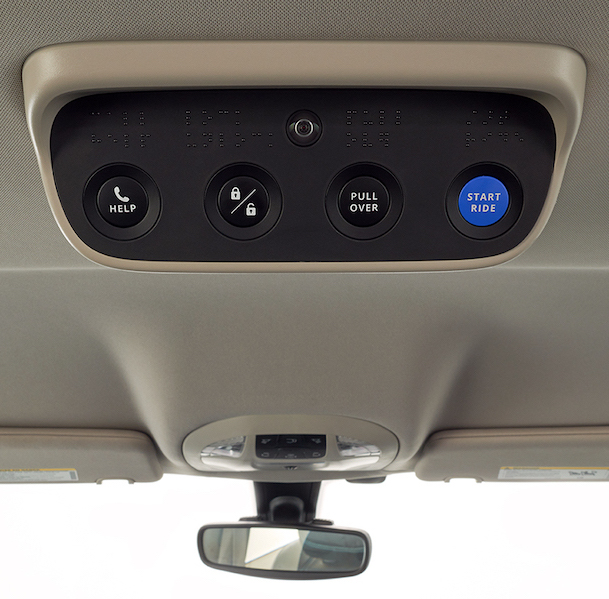
\includegraphics[height=0.27\textwidth]{fig/WaymoButtons}\hfill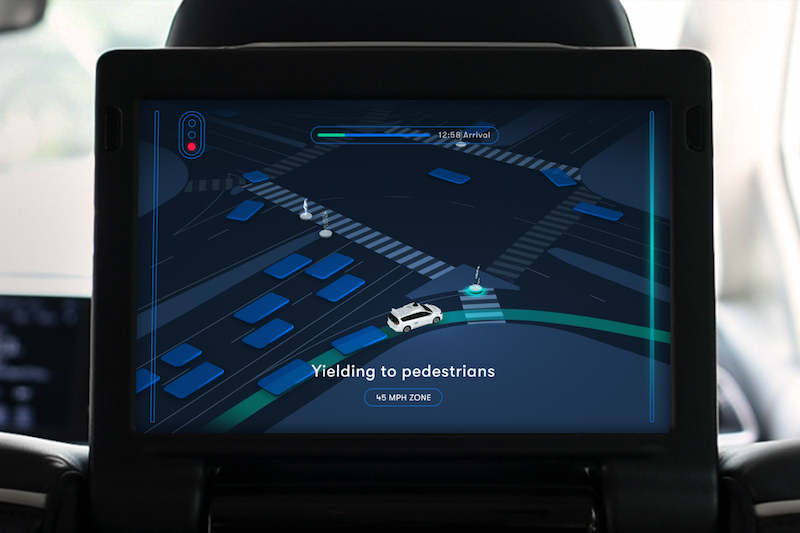
\includegraphics[height=0.27\textwidth]{fig/WaymoScreen}\hfill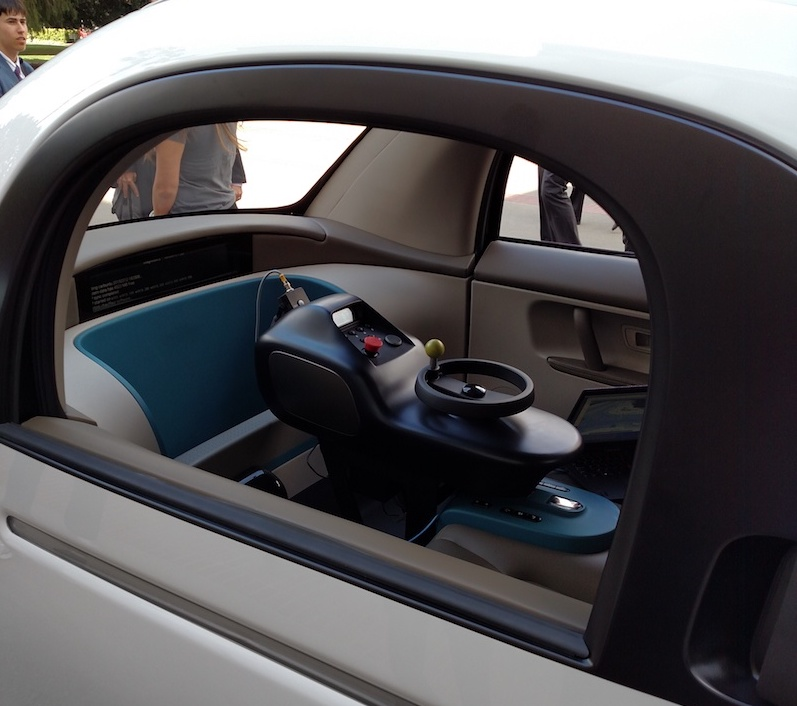
\includegraphics[height=0.27\textwidth]{fig/GoogleCar}
    \caption[Waymo autonomous vehicle interfaces]{Waymo autonomous vehicle interfaces. Images downloaded from: \url{https://arstechnica.com/cars/2017/11/fully-driverless-cars-are-here/} and \url{https://nathanpfry.com/google-self-driving-car-powered-by-carbuntu/}}
    \label{fig:fig-waymo}
\end{figure}
The vehicle interface of Waymo, the leading autonomous vehicle research company (by million autonomously driven miles), is very minimalistic. It has four buttons with braille text, a video camera and a display. The display seems to be without any touch input, the display is only used to show the route, what the vehicle detects and other sensor data (\emph{\fullref{fig:fig-waymo}, center}). The buttons allow to start the ride, pull over, lock/unlock doors and call for help (\emph{\autoref{fig:fig-waymo}, left}). The tour is planned and the vehicle is summoned by an accompanying app. 
Pictures from the older Google Car (now Waymo) show a very different interface (\emph{\autoref{fig:fig-waymo}, right}). 
It has a big stop button, a display below the windshield, a small display in front of the operation buttons and a horizontal steering wheel. Even if this interface might just be used for testing, it makes it very obvious how the newer Waymo interface tries to make driving autonomously look like nothing extraordinary. 

If we relate autonomous driving to using a cab, the software interface might look strikingly similar to those of ride-hailing services. Uber, Lyft, Mytaxi all use a map, which shows close by cabs. Furthermore, they make the user select the destination and starting point and allow to select a price category of vehicles.  

\subsection{Concept Cars}
\label{sec:conceptcars}
\begin{figure}
    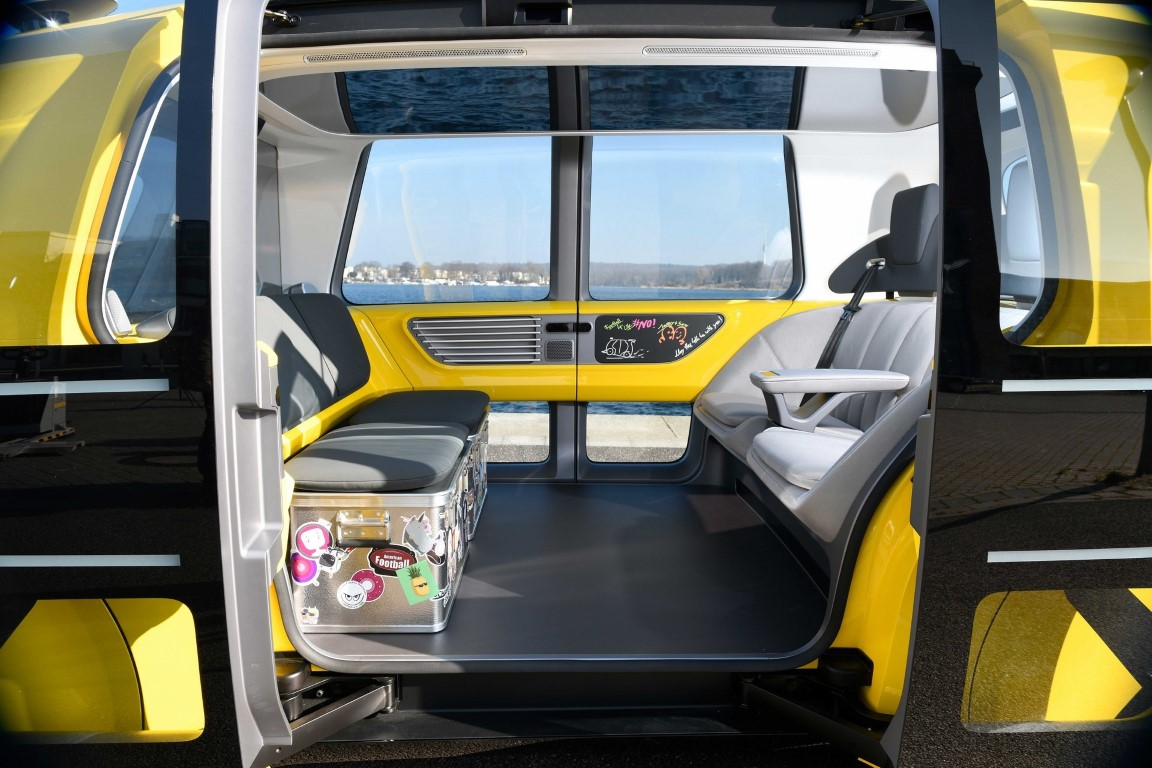
\includegraphics[height=0.2725\textwidth]{fig/school_bus_Mittel.jpg}\hfill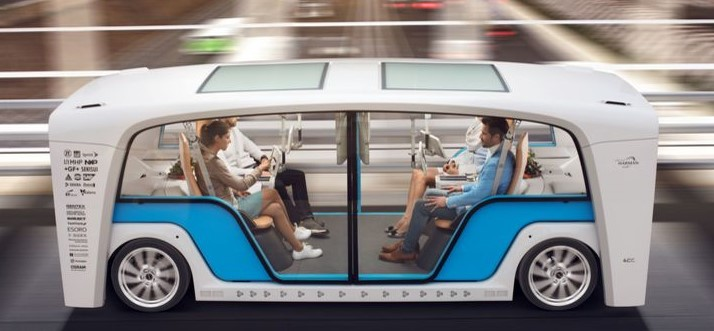
\includegraphics[height=0.2725\textwidth]{fig/snap.jpg}\newline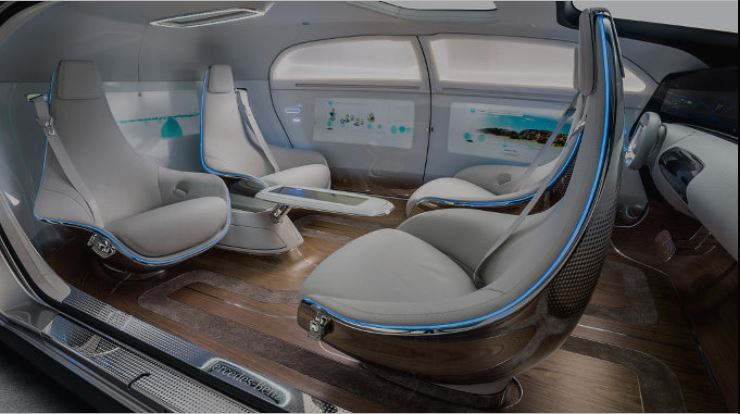
\includegraphics[height=0.28\textwidth]{fig/mercedes.JPG}\hfill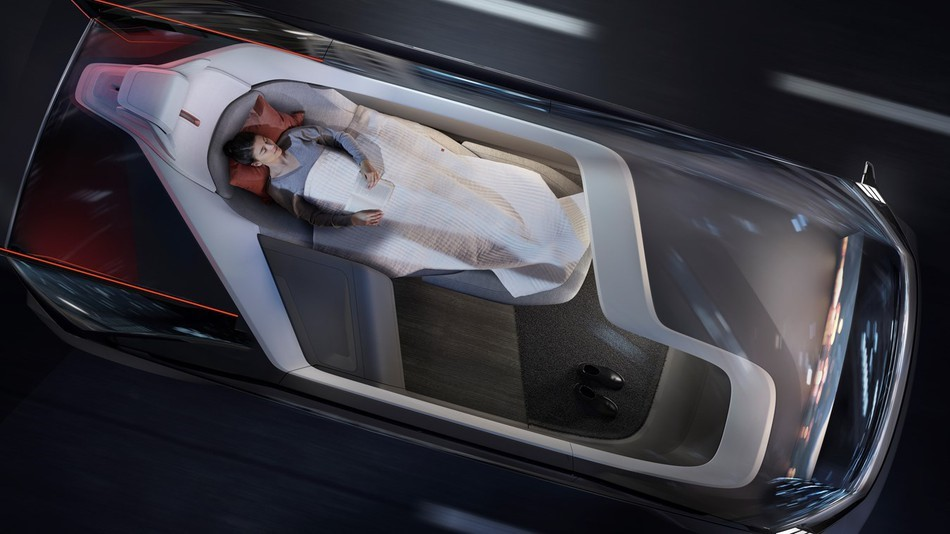
\includegraphics[height=0.28\textwidth]{fig/360c_Mittel.jpg}
    \caption[Concept Cars]{Concept cars: Sedric Schoolbus, Snap, F 015, 360c Downloaded from: \url{https://www.mercedes-benz.com/en/mercedes-benz/innovation/research-vehicle-f-015-luxury-in-motion/}, \url{discover-sedric.com/}, \url{https://www.rinspeed.eu/de/CES-Las-Vegas-2018_17_aktuelles.html} and \url{https://www.aircraftinteriorsinternational.com/news/passenger-experience/could-volvo-disrupt-domestic-air-travel.html}}
    \label{fig:conceptcars}
\end{figure}
Vehicles and vehicle concept such as the IBM Watson Olli, Volkswagen Group Sedric, Rinspeed Snap, Toyota e-Palette and Navya Autonom Shuttle show a public transport oriented design with minimalist interior and fixed simple seats. This is in stark contrast to the interfaces of personal autonomous vehicles such as the Tesla Models, Volvo Concept 6 or Mercedes-Benz F 015, cars that still have the steering wheel, dashboard and comfortable car seats and allow to retract or reverse them. The Volvo Concept 360c even has space for a bed and promotes it as an alternative to flying in the first class (\emph{\fullref{fig:conceptcars}}).   

\subsection{Pedestrian interfaces}\label{ssec:pedestrian}
One of the bigger HCI questions that need to be solved is 'how do vehicles interact with pedestrians'. Most of these communications are simple things like: 'Go ahead, I noticed you'. However to communicate these messages body gestures are necessary, which vehicles do not have the modes for. Possibilities are virtual avatars that represent the driver with, text or voice.  A clever communication method is used by the Mercedes-Benz F105, which uses a laser to beam a representation of a zebra crossing on the ground. Virginia Tech and \cite{FordMotorCompany2017FordPeople} built a prototype of an autonomous vehicle that uses a light strip to communicate with pedestrians, i.e., at a zebra crossing. Lyft cabs use a colored light pod, the amp\footnote{\url{https://take.lyft.com/amp/}}, to show to travelers which car is the one they summoned. \cite{Mahadevan2018} specifically looked into the nonverbal cues that allow pedestrians to cross roads and developed prototypes for a vehicle and Segway robot. 

\subsubsection{Communication with other vehicles} 
Communication with other drivers needs to be handled by autonomous vehicles too. Whether it is who will pass a crossing first, when in doubt, or when to honk for bad driving behavior. Interestingly, even now the possibilities to communicate with other drivers are limited. Only the headlamp flashers, the horn and turn indicators exist beside face to face communication. The Mercedes-Benz F105 has another addition, an LED text panel on the back of the vehicle. They use it to communicate that the vehicle is in autonomous mode and therefore driving slower than usual, much like vehicles from driving schools use signs to remind other drivers to be mindful.  

\subsection{Transportation-as-a-Service}\label{ssec:TaaS}
Transportation-as-a-Service (or also Mobility-as-a-Service) describes a predicted shift from vehicle ownership to renting and sharing vehicles, especially in urban areas. Even though ridesharing and carpooling was very common in the 40s and again in the 80s and 90s (in the U.S.) it declined rapidly by the 90s \citep{Ferguson}. The major reason for this decline is cheaper gas prices after the oil crises. Furthermore, cheaper vehicle costs, more spread out suburban living and improved roadway systems are the reasons for the death of carpooling. 

In urban cities, the new trend of TaaS is manifesting with ride-sharing, e-hailing services, bike-sharing programs, as well as car-sharing, all of which are enabled by the internet. In particular, improved map services and journey planners are conditions that allow users of TaaS to plan their routes individually. These services are usually available as subscription services or are 'pay as you go'. An early concept of TaaS was described by \citet{Tschanz1996TheServices}. Fully autonomous vehicles will most likely be employed as TaaS; Waymo, Uber, Lyft, and others have announced that they are working on such services and have even shown functional prototypes\footnote{\url{https://stratechery.com/2016/google-uber-and-the-evolution-of-transportation-as-a-service/}}. If autonomous vehicles are enabling ride sharing with strangers, a major concern is how to match the users of such services. The advantages of TaaS are potentially enormous: 'less time driving yourself', fewer greenhouse gases and pollutants, less traffic congestion, more random social encounters, less money spend on vehicle and vehicle maintenance and less space needed for parking lots.
Furthermore, autonomous vehicles might lead to reduced stress, improved productivity and fewer accidents \citet{Fagnant2015PreparingRecommendations}. However, whether or not autonomous vehicles will lead to less congested roads, fewer greenhouse gases are highly controversial. The reason is that an increase of comfort by autonomous vehicles might actually lead to more use of them, which in turn means that more miles are traveled\footnote{\url{http://humantransit.org/2015/11/self-driving-cars-a-coming-congestion-disaster.html}}\fnsep\footnote{\url{https://www.citylab.com/transportation/2014/04/will-world-driverless-cars-be-heaven-or-hell/8784/}}\fnsep\footnote{\url{https://www.ptua.org.au/myths/robotcar/}}. A good overview on the potential benefits and problems can be found in \citet{Litman2014AutonomousPlanning}. 

\subsection{Steering wheel}\label{ssec:steering}
\begin{figure}
   \hfill\ 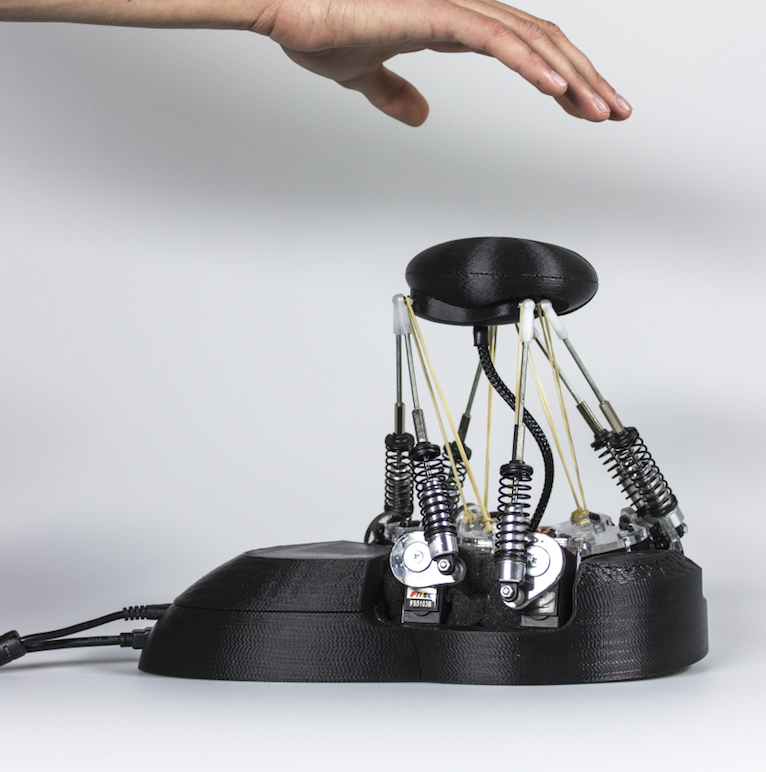
\includegraphics[width=0.4\textwidth]{fig/joystick}\hfill\
    \caption[The tactile joystick 'Stewart' for autonomous vehicles]{The tactile joystick 'Stewart' for autonomous vehicles. Image from \url{http://felixros.com/stewart.html}}
    \label{fig:joystick}
\end{figure}
Even the invention of fully electric steering, braking and pedaling, which allow the actual shape of these interfaces to be arbitrary, and the invention of assistance Systems such as autosteer and ACC did not change the general shape of the consumer driving interfaces at all. A well thought out tactile interface is that of industrial designer Felix Ross (\emph{\fullref{fig:joystick}}). It is a moving and vibrating joystick that mediates what the car is doing such as accelerating or taking turns. It is also meant to allow the driver to influence these decisions by moving the joystick. This control, however, seems more suited for self-owned autonomous vehicles where there is only one person that has order over it. In the TaaS concepts mentioned earlier, the steering wheels are left out. It might be worthwhile to explore collaborative driving interfaces further. 

\subsection{Car as a living space}\label{ssec:living}
If there is no driver in the vehicle, people could use the vehicle as their living room. This concept can be seen with car concepts that do not have seat belts anymore, are reversible or have a couch table in the center. An extreme version of this is the Hyundai Mobility Vision Concept \footnote{\url{https://www.hyundai.news/eu/technology/hyundai-motor-demonstrates-mobility-vision-with-hyper-connected-car-and-smart-house/}}, which presents a vehicle that docks physically into the living room and becomes a part of the interior. My preceding Intern  \citet{Honma2017SystemVehicles} concludes in his bachelor thesis work that there will be many different scenario dependent autonomous vehicles. For example, Disney branded vehicles that drive families to their parks or workout vehicles owned by gym chains that allow passengers to warm up before arriving at the gym. As discussed in \emph{\fullref{ssec:TaaS}} car ownership might become a thing of the past, the implication is that driving a car will become less about expressing an identity and more about “inhabiting a space” \citep{Laurier2012WhatCar}.

\subsection{Seating arrangements}\label{ssec:seating}
\begin{figure}
    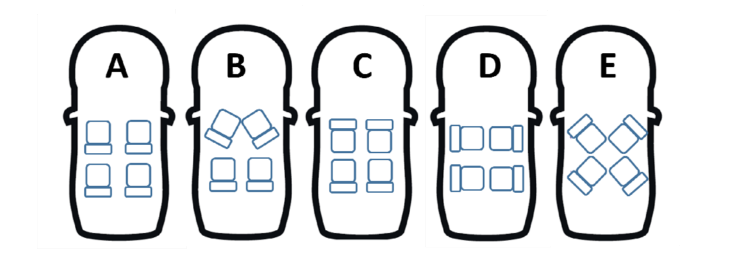
\includegraphics[width=1\textwidth]{fig/seating}\hfill\
    \caption[Seating arrangements]{Different seating arrangements in autonomous vehicles. Figure from \cite{Jorlov2017}}
    \label{fig:seating}
\end{figure}
A study of seating arrangements in autonomous vehicles from Navya\footnote{\url{http://navya.tech/en/autonom-en/autonom-cab/}}, Olli\footnote{\url{https://localmotors.com/meet-olli/}} and the Google Car reveals that they often do not have the traditional seating arrangement of consumer cars. Further concepts such as the Volvo Concept 26\footnote{\url{https://www.volvocars.com/de/modelle/concept-cars/concept-26}}, Mercedes-Benz F 015\footnote{\url{https://www.mercedes-benz.com/de/mercedes-benz/innovation/forschungsfahrzeug-f-015-luxury-in-motion/}}, or Volkswagen Group Sedric\footnote{\url{http://www.discover-sedric.com/en/}} show also very different seating arrangements.  \citet{Jungwirth2017LeadershipGroup} distinguish between autonomous vehicles for ownership, TaaS for People with Pods (vehicle for 2-6 people) or Shuttles (vehicles for more than six people) and TaaS for Goods with Urban and Highway use cases. In a qualitative study with 52 participants, \citet{Jorlov2017} explored future seating positions and activities in highly automated cars. In this study, the participants were seated on traditional chairs in front of an image of an autonomous vehicle and should imagine driving in such a vehicle. The \emph{\fullref{fig:seating}} shows the identified seating positions for longer drives with social activity. Users preferred the seating position C, followed by E and D. Even though this study is very limited in that it was conducted in a static setting and therefore no influencing factors such as car sickness or access to input devices were considered, it shows that autonomous vehicles might be a lot more dynamic in the seating arrangements.  

In highly autonomous vehicles it is not obvious who is in control and therefore not obvious where the major input and output devices will be. The ownership concepts such as Volvo Concept 26 sometimes keep the driver seat as the most important place. The steering wheel still exists, and cluster and entertainment displays are positioned to be easily accessible for the driver. The Mercedes F015 on the other hand places displays with touch input everywhere: in the cluster, in the side panels and inside of a central table. The central coffee table as a control device appears in other concepts too, such as the BOSCH CES 2015 car\footnote{\url{http://fearless-experience.com/index_neb.html}} or the Panasonic Autonomous Cabin Concept\footnote{\url{https://newatlas.com/panasonic-autonomous-cabin-concept/47280/}}. Autonomous vehicles that are more oriented towards the MaaS or public transportation often do not have any visible interfaces inside the cabin at all (See the Sedric, Olli and Renault EZ-GO\footnote{\url{https://www.renault.de/modellpalette/concept-car/ez-go-concept.html}} The Navya autonomous cab has one long vertical display such as can be found inside of subways. The control interface to summon such a vehicle is often a smartphone app instead. 

\subsection{Anthropomorphic features}
As vehicles become increasingly more intelligent and anthropomorphic, the question arises where the intellect and personality of the vehicle are located. Vehicles have an outside shell but contain the users inside them. It is well studied that vehicles are often seen as the extension of the driver's personality, that human facial features are recognized in the front end of automobiles and that people ascribe various personality traits to these \citep[see][]{Windhager2008FaceDesigns}. Some concepts of autonomous vehicles such as the Volkswagen Sedric and Smart Vision EQ Fortwo\footnote{\url{https://www.youtube.com/watch?v=fntak9UCnLs}} even animate their facial features. Vehicles of the premium range, as well as trucks and SUVs, often have masculine features as they portray speed, pleasure, control, risk-taking, and embodiment\footnote{\url{https://www.2025ad.com/latest/automated-driving-and-masculinity/}}. There is an interesting discussion by \citet{Balkmar2018} of whether autonomous vehicles might lead to a degendering and regendering of motor vehicles.
While the concept of the vehicle as a living space (\emph{\fullref{ssec:living}}) would indicate a process of deanthropomorphization, other studies point to the fact that people assign personalities and acknowledge autonomous vehicles’ humanlike intelligence \citep[see][]{Waytz2014}. An interesting thought is that because navigation system voices and other text to speech services are usually female\footnote{\url{http://www.bbc.com/autos/story/20160303-are-you-gps-gender-biased}}, would that mean that other anthropomorphic features of an autonomous vehicle have to be female as well? 

Some movies envision autonomous vehicles with a virtual cab driver (\emph{\fullref{sec:history}}). The Chinese car startup NIO has a digital assistant with simplistic facial features integrated into the console that can talk, blink and move its head. Nissan was experimenting in 2005 with a similar driving assistant (see \emph{\fullref{fig:robots}}). In a text by \citet{Perchonok2009FacilitatingLiterature} social interaction through speech and nonverbal communication with driver assistant robots are discussed. Other possibilities for visually present assistants are avatars and holograms. 
\begin{figure}
    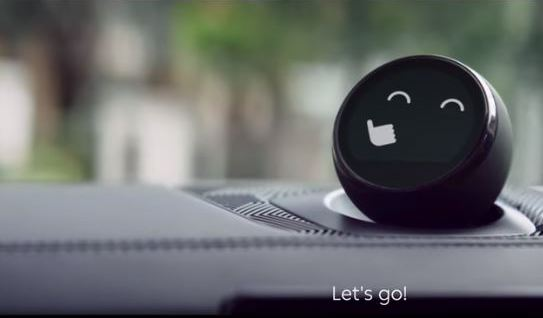
\includegraphics[height=0.28\textwidth]{fig/NOMI}\hfill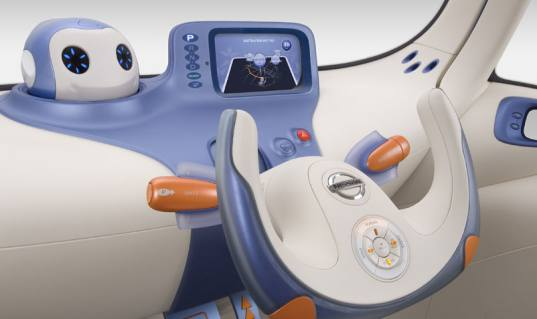
\includegraphics[height=0.28\textwidth]{fig/PIVO}
    \caption[Social Robots in Cars]{Social Robots in Cars. Left: NIO NOMI 
   Right: Nissan PIVO 2. Images downloaded from: \url{https://www.cleanthinking.de/nomi-so-sympathisch-kann-kuenstliche-intelligenz-im-auto-sein/} and adapted from \cite{Perchonok2009FacilitatingLiterature}.}
    \label{fig:robots}
\end{figure}

In my opinion there is not much use in a visually located  avatar; as of now it would suggest social intelligence, which assistants do not have yet; it would be difficult to be positioned in reach for all passengers, have issues with the uncanny valley and locate the perceived intelligence of the vehicle in one spot inside the cabin, whereas an autonomous vehicle appears as one intelligent agent on the outside. Instead, the inside of an autonomous vehicle might be compared metaphorically to a womb. A safe, comfortable place that encases the passengers and takes responsibility from them (see also \emph{\fullref{ssec:living}}). A personality and character could help autonomous vehicles to establish the initial trust people need for it to use, just as the first successful ATM had a character and voice too\footnote{\url{https://en.wikipedia.org/wiki/Tillie_the_All-Time_Teller}}.

\section{Trust Self-driving Vehicles}\label{sec:trust}
Most fatalities (94\%) on the road can be traced back to human error \citep[see][]{Singh2015CriticalSurvey}. Only a few accidents occur because of technical flaws. Therefore, the most dangerous aspect of being in a vehicle is the driving behavior. If a human hands over operation of the vehicle to an autonomous system he needs to trust that it performs the driving task equally well. 

A study by \citet{Hauslschmid2017} investigated if three different visualizations could enhance trust in autonomous driving: a chauffeur avatar, a world in miniature and a display of the vehicles indicator lights. These visualizations reacted to four different situations (turn, close objects, traffic lights, and danger) and were presented on a head-up display in a self-built driving simulator. As opposed to the researchers' hypothesis the subjects rated the world-in-miniature higher in trust than the anthropomorphic chauffeur avatar. They hypothesize that the miniature world conveys a stronger feeling of competence and is, therefore, more suitable to the technical system than a human-like visualization.

Contrary to this finding \citet{Waytz2014} found that anthropomorphism (as measured by the subjects impression of how smart the car was, how well it could feel what was happening around it, how well it could anticipate what was about to happen and how well it could plan a route) increased trust in the vehicle. Moreover, participants were more relaxed in an accident and blamed their vehicle and related entities less for an accident caused by another driver in the anthropomorphic condition. The anthropomorphic features given to the vehicle in this study were the name, gender, and voice. 
In a study by \cite{Korber2018}, participants were manipulated in their trust before a semi-autonomous simulator drive. People in the trust promoted group scanned the environment less, spent more time on a non-driving related task and were more likely to crash into an obstacle. 
A study by \citet{Beattie} found that participants in a car simulator study felt more in control when autonomous vehicles communicated their driving decisions by spatial sounds as opposed to no sound feedback. The sounds they used in this study were recordings from real vehicles (acceleration, braking, gear changing, clutch, indicator, and ignition). Research by \citet{Helldin2013PresentingDriving} suggests that too high levels of trust can lead to dangerous over-reliance on autonomous cars. The authors found that their UI, which communicates the certainty of the autonomous car allows passengers to calibrate trust in the system and react more safely. 

In an ethnographic study over six days \citet{Lee2016} summarize dimensions underlying trust but as the authors suggest: more importantly on distrust.  Findings of this ethnographic study are that all passengers participating in this study felt anxious when they were not adequately informed, especially about future actions. Also, unpredictable events, such as somebody running in front of the vehicle, were worrying to participants; participants felt irritated by the robotic movement of the steering wheel and mentioned that they might prefer not to be able to see it turning. Finally, participants were positively influenced by trust if they saw a purpose in autonomous vehicles or negatively influenced by social factors, such as taxi drivers who will lose their jobs because of automation. The authors summarize that in order to enrich driving experiences in automated cars, it would be essential to identify the factors that cause distrust and transform them into positive experiences rather than emphasizing trust factors. 

\subsubsection{Trust autonomous robots}
Vehicles that drive autonomously are a type of robots. It might be beneficial to apply research knowledge from human-robot interaction to autonomous vehicles. There is an argument that a shift from vehicles as tools towards vehicles as intelligent agents is happening \citep{Thill}. Since robots are difficult to compare, robotics researcher \cite{Steinfeld2006}, try to identify common metrics that allow comparison of social robots among different applications. For social robots, those are interaction characteristics, persuasiveness, trust, engagement, and compliance. 

\section{Study Autonomous Vehicles}\label{sec:studies}
Waymo, the most visible developer of autonomous vehicles, praises itself for designing autonomous vehicles not just to be inclusive but to be developed for the disabled preeminently \citep{Waymo2018DriverlessApplication}. Even though developers seem to focus already on the importance of the User Experience, there are no common guidelines or measures for evaluating autonomous vehicles. In \emph{\fullref{ssec:living}} the idea of the vehicle as a living room was established and in \emph{\fullref{sec:trust}} trust was discussed; therefore the two most important emotional measures of an autonomous vehicle may be trust and comfort.  

A big issue is the lack of access to autonomous vehicles, especially fully autonomous vehicles of SAE 3 and up. Most autonomous vehicles employ a whole range of sensors and especially LIDAR sensors are still expensive\footnote{\url{http://www.latimes.com/business/la-fi-hy-ouster-lidar-20171211-htmlstory.html}}. Even at companies such as BOSCH, which do have autonomous vehicles, access to them is restricted as they are almost nonstop in use for testing by the self-driving vehicle groups. Even if researchers can get access to an autonomous vehicle, most likely it is only borrowed for a short amount of time, and therefore complex modifications of the vehicle or implementation of prototypes into the vehicles are difficult. Then, most states only issue licenses that require a safety driver and occupants to be employed by the autonomous vehicle manufacturer \citep[see][]{Jones2013AutonomousReport}. 

Therefore, studies of autonomous vehicles often use lower level autonomous vehicles or are of short duration. 
Most published user research in vehicle interaction uses car simulators as they allow for highly controlled experiments, which are needed for experiments with internal validity. To increase the external validity of simulators some of them are paying extreme attention to details. For example, the interior of the vehicle is as close as possible to those of real vehicles and multiple sensors, speakers, projectors, and actuators replicate effects that occur during rides. These simulators proofed to be valuable for studies that focus on many aspects while driving, such as safety: i.e., it allows to measure reaction times accurately. 

However, a lot of important aspects of user research in autonomous vehicles cannot be recreated in simulators. Loss of control and lack of trust in the autonomous system are inhibitors (see \emph{\fullref{sec:trust}}) against the use of autonomous vehicles, it is difficult, if not impossible to recreate these aspects in simulators. Once test subjects enter a simulator, they know that they are part of a controlled experiment and if a simulated accident occurs, it would not be of any harm. Consequently, immersion and presence are lost. Perception of danger and immersion are lower, and moreover, sleepiness is higher in a simulator than in a real car \citep{Hallvig2013}.
Simulators are optimized to recreate the experience of driving, which means that the driving inputs such as steering and braking are simulated well. Even though some simulators have moving cabins, the inertial and vestibular cues, which are needed for distance perception are weakly recreated. Evaluating perception in driving simulation experiment, are challenging to recreate closely. Passengers are usually not researched, and therefore, most driving simulators do not even have back seats (see \emph{\fullref{fig:simulators}}). To sum up, simulators study often suffer from ecological validity, which might negatively influence the external validity of experiments. 

\subsection{On the road driving simulators}\label{ssec:simulator}
\begin{figure}
    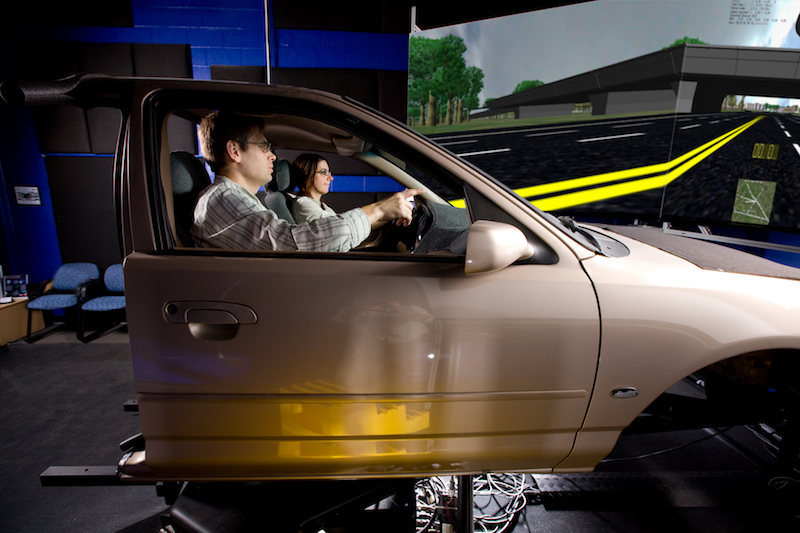
\includegraphics[height=0.3\textwidth]{fig/simulator}\hfill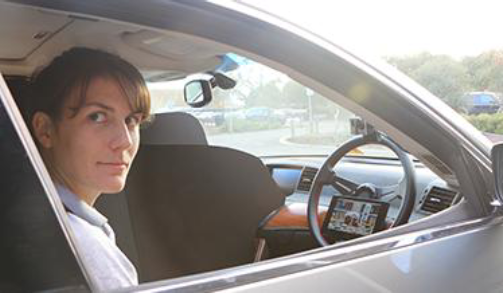
\includegraphics[height=0.3\textwidth]{fig/rrads}
    \caption[Driving simulators]{Left: Driving simulator of the University at Buffalo. 
   Right: The Real Road Autonomous Driving Simulator. Images downloaded from: \url{http://www.buffalo.edu/news/releases/2008/12/9819.html} and adapted from \citet{Baltodano2015}}
    \label{fig:simulators}
\end{figure}
Interesting approaches of on the road \emph{Wizard of Oz} experiments have sprung up recently.  WOz studies are sometimes criticized for their validity and use of deception\citep[see][]{Riek2012WizardGuidelines}. However, testing the user experience of real humans in close to real-world scenarios is often not possible otherwise. 

The Real Road Autonomous Driving Simulator by\citet{Baltodano2015} uses a partition to separate the test subject on the front passenger seat from the actual driver (see \emph{\fullref{fig:simulators}}). Even though the researchers do not use overt deception, some participants believed that they were riding in a real autonomous vehicle. This platform allows to test prototypes quickly and might be very effective to study handover scenarios. Indeed a similar system was developed to test exactly such scenarios: Marionette by \citet{Wang2017} is specifically designed to allow the test of semi-autonomous systems. It uses a right-handed driving vehicle so that participants can sit in the left seat, which is in most countries the driver's seat. Furthermore, it uses a gamer driving wheel for feedback but also a possibility of intervention. If the test subject steers accelerate or brakes with the gaming wheel or pedals, LED signals show the driving wizard what the test subject is doing: e.g., steering left or braking. He can then recreate these driving decisions with the real driving controls. During the ride study participant as well as the context for each drive are recorded because of the variability between each participants test drive. 

Another interesting approach is VR-OOM by \citet{Goedicke2018}, an on-road VR driving simulator. The researchers make the test subjects sit in a real vehicle, which drives over an open area such as a parking lot. The vehicle is steered by a driving wizard and additionally controlled by another interaction wizard; the test subject wears a VR headset, has gaming steering wheels and pedals in front of him and sees a virtual car and road while feeling the actual motion of the vehicle. For this approach, the virtual and physical location of the vehicles is synchronized. This approach allows testing a few other use cases that might not be possible in another setting. Still, the size of the parking lot restricts this setup, longer driving studies are not possible. Subjects will stay aware that what they see is fake, which impairs the feeling of presence. 
To test the interaction of pedestrians with autonomous vehicles \citet{FordMotorCompany2017FordPeople} and \citet{Rothenbucher2016} covered the driver with a vehicle seat costume. This allows testing how pedestrians interact with vehicles as if there are no driver insights. 

\subsection{No eye contact}
These on the road Wizard of Oz experiments do not use overt deception but disconnect the test subject from the driver. I argue that for testing human-machine interaction with autonomous vehicles it is important that the test subjects feel that they are on their own. If they see that there is another researcher (e.g., the interaction wizard) in the vehicle they might already have an initial trust in the whole autonomous system right from the start. If they can make eye contact with a researcher, they might establish empathy with the researcher \citep[see][]{Haase1972NonverbalCommunication}, and this could overshadow the trust of the test subject into the system. If there were any inconvenient or dangerous situations, they could always rely on them, a person with competence, as a backup. Therefore, it is important that the test subject can neither establish eye contact with a researcher in the vehicle nor a driver. We know that taxi drivers employ multiple strategies to build trust with their customers \citep[see][]{Gambetta2005Streetwise} and we are interested in the trust of the test subject into the “autonomous system” not of that into the researcher. Furthermore, some passengers show “back-seat driver” behavior if they are not driving themselves\footnote{\url{https://www.psychologytoday.com/us/articles/201005/field-guide-the-backseat-driver-pedal-the-meddle}}. It is important to investigate how this type of people feel if they are not in control of themselves and also cannot perceive how the vehicle is driving from gestures and sight of a human. 

\subsection{UX Factors}
\label{ssec:UXfactors}
The importance of the Users Experience in Interface Design has become acknowledged \citep{Soegaard2013TheEd.}. Some important measures of user experience in autonomous driving simulators were identified by \cite{Ive}. The following is an adaption for real road driving simulators: 

\begin{itemize*} 
  \item Trust in technology and automated systems\quad
  \item Plausibility of the (self) driving scenario\quad
  \item Car sickness\quad
  \item Comfort\quad
  \item Driver profiling\quad
  \item Need for control\quad
  \item Sensation seeking\quad
  \item Needs\quad
  \item Emotional response\quad
  \item Perceived quality\quad
\end{itemize*}

Compared to \cite{Ive} measures the following were changed: \emph{Measuring Presence in a Virtual Environment} is not required for real road driving simulators; however, the plausibility and convincingness of the wizard of oz setup are of importance. \emph{Simulator Sickness} won't occur in a real road driving simulator, however, car sickness does. For fully autonomous systems (without hand-over scenarios) \emph{sleepiness} is of lower importance though low alertness could indicate high trust in a vehicle. As argued in \emph{\fullref{sec:trust}} comfort might be of the most important UX factors for fully autonomous vehicles. Therefore, sleepiness was exchanged for comfort. To measure comfort or relaxation, possibly physiological measures can be taken into consideration. For example, the absence of stress indicates relaxation \citep{Salai2016}. \emph{Driver profiling} should focus not on the driving style (e.g., driver’s skill level) but on co-driver behavior (e.g., if passengers are used to be back-seat drivers). \cite{Burger1979TheControl} scale could measure the 'need for control' of an individual.

\subsection{Car sickness}
\label{ssec:carsickness}
One of the major selling points of autonomous vehicles for the average driver is the expectation that they can free up driving time for more valuable activities. However, car sickness is a strong inhibitor against that argument. Individuals' suffering from car sickness varies greatly but most people are not able to read books during drives. Motion sickness is most frequently caused by the conflict between visual and vestibular inputs; these critical conflicts will increase with improving image quality of onboard displays \citep{Diels2016}.

Further, loss of control over one’s movements and reduced ability to anticipate the direction of movement are also reasons for motion sickness \citep{Sivak2015}. The major car-sickness inducing movements are associated with horizontal accelerations caused by accelerating, braking, and cornering \citep{Diels2016}. These effects are more commonly experienced by passengers than the driver which explains why drivers suffer less often from car sickness. Narrow, opaque or small windows, non-forward gaze, and side or rear facing posture all worsen car sickness. Having the eyes closed, a supine posture and being asleep help \citep{Sivak2015}. Hence, the seating positions identified in \emph{\fullref{ssec:seating}} are possible causes of car sickness. 

People use various strategies against car sickness, one of the most important is to look out of the window regularly\footnote{\url{https://www.wikihow.com/Avoid-Nausea-when-Reading-in-the-Car}}, and to have the head higher up: \citet{Kuiper2018LookingCarsickness} used the MISC scale (by \citet{Bos2005MotionView}) and found that higher placed in car displays are beneficial against car sickness. In addition, motion sickness is related to the ability to anticipate the future motion path on the basis of motoric and visual information, which can also be provided via artificial enhancement of the visual scene: to measure air sickness in planes \cite{Feenstra2011AAirsickness} used MISC and JOSC self-reported measurement scales and showed that artificial moving visual images could be used to reduce motion sickness and thereby improve comfort.

\subsection{Data}
\label{sec:Data}
Self-driving vehicles need much data. Two of the most prominent companies have easy access to it: Tesla vehicles collect them from their customers while driving on the road and Google collects them from users of their Google Maps navigation software and also do they employ a huge array of mapping vehicles for their Maps service. An open source approach of data collection is used by comma.ai, a small company that sells OBD dongles that connect to the vehicle and a smartphone camera to connect driving data from their users \footnote{\url{https://medium.com/@comma_ai/a-panda-and-a-cabana-how-to-get-started-car-hacking-with-comma-ai-b5e46fae8646}}. While most data that autonomous car researchers are interested in is road data from LIDAR, radar and photo cameras, the steering, braking, and acceleration behavior of humans is also of interest. A naturalistic driving study by MIT goes even further \cite{Fridman2017MITAutomation} and collects additionally several data points which are of high interest for HCI research from the driver (video recordings of the cabin, interviews, and questionnaires). 

\section {The Best Interface is No Interface}
\label{sec:nointerface}
Golden \citeauthor{krishna2015best}'s book \emph{The Best Interface Is No Interface} \citeyear{krishna2015best}  provides an important line of thoughts. His major concern is that with the internet of things and smart homes devices that traditionally did a good job without any interface got “a screen slapped on it”. There is refrigerators, trash bins, microwaves that have big touch screens attached to them and often do nothing else with it then show time or weather. Even vehicles infotainment systems started to get problematic features such as checking Facebook or Twitter in the instrument cluster. Some new interfaces such as Amazon Alexa and Google Assistant do not even have a screen at all. For great experiences, designers need to consider the User Experience (\emph{\fullref{ssec:UXfactors}}). 
 
I agree that too many displays and input options inside vehicles are not just useless but also defy the purpose of great UX. Moreover, I do think that vehicle manufacturers should not try to compete with brought in devices. An iPhone or Nintendo Switch will always provide better entertainment than, e.g., a solitaire game embedded into a coffee table display developed by a car manufacturer. Instead, vehicle manufacturers and OEMs should focus on enabling these devices by providing enough power plugs, fast internet or a movie database from which passengers can stream movies. Ambient displays are a great example of interfaces without an interface (\emph{\fullref{ssec:ambient}}). 